\chapter{Introduction}

The amount of information that people are exposed to can be daunting and the amount of options to choose from can simply be overwhelming. Consequently, it has become incredibly demanding to choose interesting and relevant content across a broad range of choices. For example, 24,000 songs are created every day, which means that about one million tracks are created every six weeks. With millions of songs to choose from, it is not easy to find something new and exciting to listen to. Users face the same conundrum in many areas. 
A recommendation system is a model that can predict what users may be interested in. In essence, it is a decision-making system that helps users find personalized, interesting options, in a situation where there is an overabundance of different choices 
available. There is a clear need for good personalized recommender systems. 
The purpose of Personalized Recommender Systems is to help users navigate the  decision-making process helping them select items that are both meaningful and satisfying to them.
Current recommender systems consistently face one or more of the following problems: 1) The filter bubble problem (also called the algorithmic bias and feedback loop problem ), which refers to the phenomenon when a user receives recommendations of only familiar items, causing boredom and dissatisfaction. Most existing systems cause the model to act greedily favoring items already engaged by the user. This is particularly harmful in personalized ads recommendations as it can cause new campaigns to remain unexplored. 2) The cold-start problem, which is a condition where the circumstances  with new users and/or new items are unfavorable for the recommender system to yield the best possible results. The term ‘cold start’ derives from automobiles. When the engine is cold, cars have difficulty starting up, but they have no problems running once the engine reaches its optimal temperature. The same problem can be applied to recommender systems. Furthermore, cold starts can be classified into two distinct subsets: product cold starts and user cold starts. 3) Data sparsity refers to a computational problem  when user-item historical data is sparse. Such data is stored using a sparse matrix representation recording only the non-zeros. There is a need for an algorithm that is able to interpret sparsely represented data. 4) The problem of capturing dynamic user preferences has not been successfully handled in most current recommender systems. Traditionally recommender systems have modeled the user-item interactions in a static way capturing only a user’s general preferences. However, user-item interactions are dynamic in nature and therefore the sequential dependencies need to be taken into account to represent the current as well as recent user preferences for better and more accurate recommendations. This thesis explores five recent and alternative personalized recommender systems, which offer solutions to one or more of the aforementioned challenges. Chapter 2 provides an overview of the five different architectures covered in this thesis as well as related work. Chapters 3 through 6 delve deeper into the problems and solutions that each model provides. Finally, chapter 7 concludes the thesis.
% "PURS: Personalized Unexpected Recommender System for Improving User Satisfaction "[1] and "A Framework for Recommending Accurate and Diverse Items Using Bayesian Graph Convolutional Neural Networks" [2] focus their efforts on bringing new items to the user. The terms unexpectedness and diversity in these papers refer to the novelty of the recommendations. Moreover, "Deep Bayesian Bandits: Exploring in Online Personalized Recommendations"[3] and  "A Framework for Recommending Accurate and Diverse Items Using Bayesian Graph Convolutional Neural Networks" pay special attention to tackling the uncertainties of user-item interactions. Moreover,
% PURS and "Deep Bayesian Bandits: Exploring in Online Personalized Recommendations" both seek to overcome algorithmic bias. Furthermore, "Learning from Cross-Modal Behavior Dynamics with Graph-Regularized Neural Contextual Bandit"[4],  "A Framework for Recommending Accurate and Diverse Items Using Bayesian Graph Convolutional Neural Networks" are respectable addresses the cold-start problem faced by current personalized recommender algorithms. "Cold-start" refers to the problem with new users and/or new items causing the circumstances to be unfavorable for the recommender system to yield the best possible results.  A recent development in the area of personalized algorithms is the incorporation of the self-attention mechanism into the models. One such notable algorithm is "SSE-PT:
% Sequential Recommendation Via Personalized Transformer" [5]. All five models introduced in this paper attempt to make personalized recommendations more accurate, improving user satisfaction, and achieving state-of-the-art results. 



% \section{Related Work}
% Various personalized recommender frameworks have been proposed to resolve the problem of filter bubbles and user boredom. One noteworthy attempt at improving novelty measures includes Serendipitous Personalized Ranking described in detail in "Serendipitous personalized ranking for top-n recommendations" by Lu et al. in 2012. Deep Learning (DL) based recommender models are able to extract user preferences and make recommendations. "Deep Learning based recommender system: a survey and new perspectives" by Zhang et al. in 2019 gives an overview of current DL based recommender systems. For example, "Heterogeneous Information Network Embedding for Recommendation" by Shi et al. in 2018 presents such a model. Contextual bandits have emerged as a viable solution to address the cold-start problem faced by many recommender systems. Two such attempts  have been presented in the following works: "Latent contextual bandit and their application to personalized recommendations for new users" by Zhou et al. in 2016 and "Explore, exploit, and explain: personalizing explainable recommendations with bandits" by McInerney et al. in 2018. In addition, "Learning hidden features for contextual bandits" by Wang et al. in 2016 is an attempt to model user-item interactions using a contextual bandit algorithm. A recent research, "Deep Bayesian Bandits Showdown: An Empirical Comparison of Bayesian Deep Networks for Thompson Sampling [3], explores deep Bayesian bandit methods. Likewise, "Deep reinforcement learning based recommendation with explicit user-items interactions modeling by Liu et al. in 2018 looks into how to model long-term rewards capturing both the dynamic adaptation of user preferences as well as the interactive relationships between a user and a recommender system. The paper will be reviewed in this thesis. Likewise "Learning from Cross-Modal Behavior Dynamics with Graph-Regularized Neural Contextual Bandit" relies on contextual bandits building a Graph Regularized Cross-modal learning model (also referred to in this thesis). Recently graph convolutional neural networks (GNN) have been successful. Some notable research on the topic include "Graph Convolutional Matrix Completion by Van Den Berg et al. in 2018, "Neural Graph Collaborative Filtering by Xiang et al. in 2019, and Graph Convolutional Neural Networks for Web-Scale Recommender Systems by Ying et al. in 2018. As an example of a web-scale recommender, Pinterest proposed PinSage [10]  \textit{which is a large-scale GNN based recommender, which learns the embeddings from the pin-board bipartite graph, boosting Pinterests recommender system.} Furthermore, Natural Language Processing (NLP) literature has inspired deep learning techniques which have been harnessed to keep track of sequential data. Item sequences, equivalent to word sentences in NLP, can be modelled by attention models. The neural machine learning model, Transformer, is described in detail in "Attention is all you need" by Waswani et al. in 2017 utilizes an encoder architecture emulated by an increasing number of personalized recommender systems. One recent model motivated by the  Transformer model with state-of-the-art performance is SASRec, which is described in the paper "Self-Attentive Sequential Recommendation" by Kang et al. in 2018. 
\chapter{Model Comparison}
\section{Five Recommender Systems}
The Personalized Unexpected Recommender System (PURS), generates unexpected recommendations.  Unexpectedness is calculated as the distance between new items and user interest clusters. The Bayesian Graph Collaborative Filtering framework (BGCF) is based on Bayesian Graph Neural Networks and the node copying graph generative method which addresses the uncertainty in the underlying user-item relationship graph resulting in increased diversity to the recommendations and mitigating the data sparsity problem. The Graph-Regularized Cross-modal learning framework (GRC) addresses the challenges of representing complex non-linear user-item interactions. The system utilizes both positive and negative user-item interactions as well as unrecommended items. Moreover, many existing recommender systems use mostly historical data leading to cold-start problems for new users with no user history. Implementing neural contextual bandits, the GRC model substantially improves the cold-start performance. The Deep Bayesian bandit model attempts to reduce algorithmic bias and to optimize for long-term rewards by exploring a combination of bandit algorithms and deep neural networks. The proposed model implements a hybrid method combining the notions of bootstrapping and dropout, containing dropout units only in the second-to-last layer, and acting as "heads” in a multihead network.
SSE-PT Personalized Transformer, a neural network based model,  considers the temporal collaborative ranking problem. Owing to its attention mechanism, the system is capable of paying attention to recent items in long sequences.
\section{Comparison of Personalized Recommenders}
\begin{table}[h!]
\centering
\begin{tabular}{||c c c c c||} 
\hline
 Model & Self-Attention & Multi-armed bandits & Neural Network  & Sequential \\ [0.5ex] 
 \hline\hline
PURS & \checkmark &\xmark & DNN *&\checkmark \\ 
BGCF & \checkmark &  \xmark & GCN* & \xmark \\
GRC &  \xmark  &\checkmark &  MLP* &  \checkmark\\
Deep Bayesian* & \xmark  & \checkmark & Wide-and-Deep& \xmark \\
SSE-PT &  \checkmark &\xmark  & Transformer  & \checkmark \\ [1ex] 
 \hline
\end{tabular}
\caption{Architectural differences of Personalized Recommender Systems }
\label{table:1}
\end{table}
\begin{table}[h!]
\centering
\begin{tabular}{|| c c c c  ||} 
\hline
 Model & Accurate & Cold-Start & Feedback Loop \\ [0.5ex] 
 \hline\hline
PURS & \checkmark &   \xmark& \checkmark\\ 
BGCF  & \checkmark & \checkmark&  \checkmark \\
GRC &\checkmark  &\checkmark& \xmark \\
Deep Bayesian* & \xmark & \xmark& \checkmark\\
SSE-PT& \checkmark &\xmark &\xmark\\ [1ex] 
 \hline
\end{tabular}
\caption{The advantages and disadvantages of Personalized Recommender Systems}
\label{table:1}
\end{table}

The five recommender models explored in this paper have differences and similarities in their architectural features. As seen in table 3.1, PURS, BGCF, and SSE-PT use self-attention to extract relevant information. GRC and Deep Bayesian Bandits Algorithm make use of multi-armed bandits to find optimal recommendations. All five systems are based on some kind of neural network. PURS utilizes a Deep Neural Network (DNN) model. BGCF employs a Graph Convolutional Network (GCN) model. GRC is developed on a Multilayer Perceptron Neural Network model which is a class of feedforward artificial neural network (ANN). Deep Bayesian Bandits Algorithm (Deep Bayesian) implements a Wide-and-Deep neural network model. And finally, SSE-PT exploits a Transformer Network based structure. Three of the models, PURS, GRC, and SSE-PT, integrate sequential(temporal) user behavior. Traditionally recommender systems have modeled the user-item interactions in a static manner capturing only a user's general preferences. However, user-item interactions are dynamic and therefore the sequential dependencies need to be taken into account to represent the current as well as recent user preferences. Temporal information can be used to discover additional behavioral patterns for individual users which can in turn be leveraged to improve recommendations.

In terms of performance, it is not possible to compare the five models side by side because the evaluation metrics, the types of experiments conducted on the models, and the datasets used differ significantly. However, it is possible to look at certain performance gains for each model based on what is explicitly stated on each paper. All of the five models are scalable for large-scale real-world applications and outperform their baseline counterparts in terms of efficiency. PURS, BGCF, GRC, and SSE-PT achieve more accurate recommendations than their baselines. Three of the models, PURS, BGCF, and Deep Bayesian, emphasize novelty in their recommendations and attempt to fix the feedback loop problem. Two of the models, BGCF and GRC, implement techniques to alleviate the cold-start problem.  Overall, all of the five models perform quite well. 

\chapter{Unexpected Diverse Items}
\section{PURS Personalized Unexpected Recommender System}

The article “PURS: Personalized Unexpected Recommender System for Improving User Satisfaction” introduces a novel unexpected recommender system [1]. The motivation for developing a new approach for a recommender system is that classical recommender system methods run into the filter bubble problem when a user receives recommendations of only familiar items, causing boredom and dissatisfaction. A filter bubble is a feedback loop that users get when they use a personalized recommender system. There is a clear need for an unexpected recommender system with an element of surprise.
Unfortunately, most of the unexpected recommender systems have not been successful in real life business scenarios for the following reasons: First, the previous models have often neglected the business-oriented metrics, like  Click-Through-Rate(CTR) and Gross-Merchandise-Volume (GMV). Second, most of these models do not scale for large scale industrial applications. Third, they lack personalization, which in turn detract from user satisfaction. To overcome these problems, the researchers propose the Personalized Unexpected Recommender System (PURS) that incorporates unexpectedness into recommendations. The researchers put forward a novel deep-learning based unexpected recommender system which provides personalized and session-based unexpected recommendations. More specifically, to address this filter bubble problem, their project proposes a system that recommends items that significantly differ from user expectations, surprising them with previously unexplored items. The authors define unexpectedness as follows: "Unexpectedness of a new item as the distance between the embedding of that item and the closure of user interests in the latent space[6]." 
	
Unexpectedness leads to a notable increase in user satisfaction. Consequently, PURS optimizes the unexpectedness metric. Their proposed system is based on providing multi-cluster modeling of a user’s interests in the latent space and achieving personalized unexpectedness through implementing the self-attention mechanism and a suitable unexpected activation function. Optimization matters because if unexpectedness is overemphasized, the
recommender system will recommend items with extremely high unexpectedness, which are likely to be unimportant or even ridiculous to the user. The objective is to provide unexpected but relevant and useful recommendations. Consequently, their utility function incorporates unexpectedness into classical models, combining it with relevancy. The level of unexpectedness is adjusted to make sure that click-through rate (CTR) is maintained at a specific level while introducing unexpectedness. 
User preferences are inferred from historic behaviors. More concretely, in order to attain relevance, the most recent user actions in the window are extracted serving as the input to the MLP network. Further, user and item data is represented in the form of embeddings in the latent space and the deep-learning based autoencoder approach is implemented to procure these embeddings. 
To capture the diversity of the extracted historic user behavior,  a local activation unit able to compute the relevance of past behaviors towards potential recommendations is deployed. More concretely, the researchers apply sequence modeling and the self-attentive gated recurrent unit (GRU) neural networks to obtain the sequence embeddings. These embeddings represent personalized and session-based user perception of unexpectedness. Moreover, GRU is computationally more efficient and better able to extract semantic relationships than other recurrent models, such as long short-term memory (LSTM).
Tensorflow is used as the backend while testing PURS on three real-world datasets: the Yelp Challenge Dataset 2, containing check-in information of users and restaurants; the MovieLens Dataset 3, containing informations of users, movies and ratings; and the Youku dataset collected from the major online video platform Youku, containing information of users, videos, clicks and their corresponding features. To show that the PURS model provides unexpected and useful recommendations, they choose eight state-of-the-art baseline models. \footnote { 1) DIN Deep Interest Network designs a local activation unit to adaptively learn the representation of user interests from historical behaviors with respect to a certain item. 2) DeepFM combines the power of factorization machines for recommendation and deep learning for feature learning in a new neural network architecture. 3) Wide \& Deep Wide \& Deep utilizes the wide model to handle the manually designed cross product features, and the deep model to extract nonlinear relations among features. 4) PNN Product-based Neural Network model introduces an additional product layer to serve as the feature extractor. 5) SPR Serendipitous Personalized Ranking extends traditional personalized ranking methods by considering item popularity in AUC optimization. 6) Auralist is a personalized recommendation system that balances between the desired goals of accuracy, diversity, novelty and serendipity simultaneously. 7) DPP The Determinantal Point Process utilizes a fast greedy MAP inference approach to generate relevant and diverse recommendations. 8) HOM-LIN HOM-LIN is the state-of-the-art unexpected recommendation algorithm, which provides recommendations through the hybrid utility function for comparison.} As seen in Table 3.1, the PURS model consistently and significantly outperforms all of the baselines in both accuracy and as well as unexpectedness. Furthermore, they also show that all deep-learning based approaches perform much better than feature-based methods, illustrating the effectiveness of latent models.
\begin{table}[ht!]
    \centering
    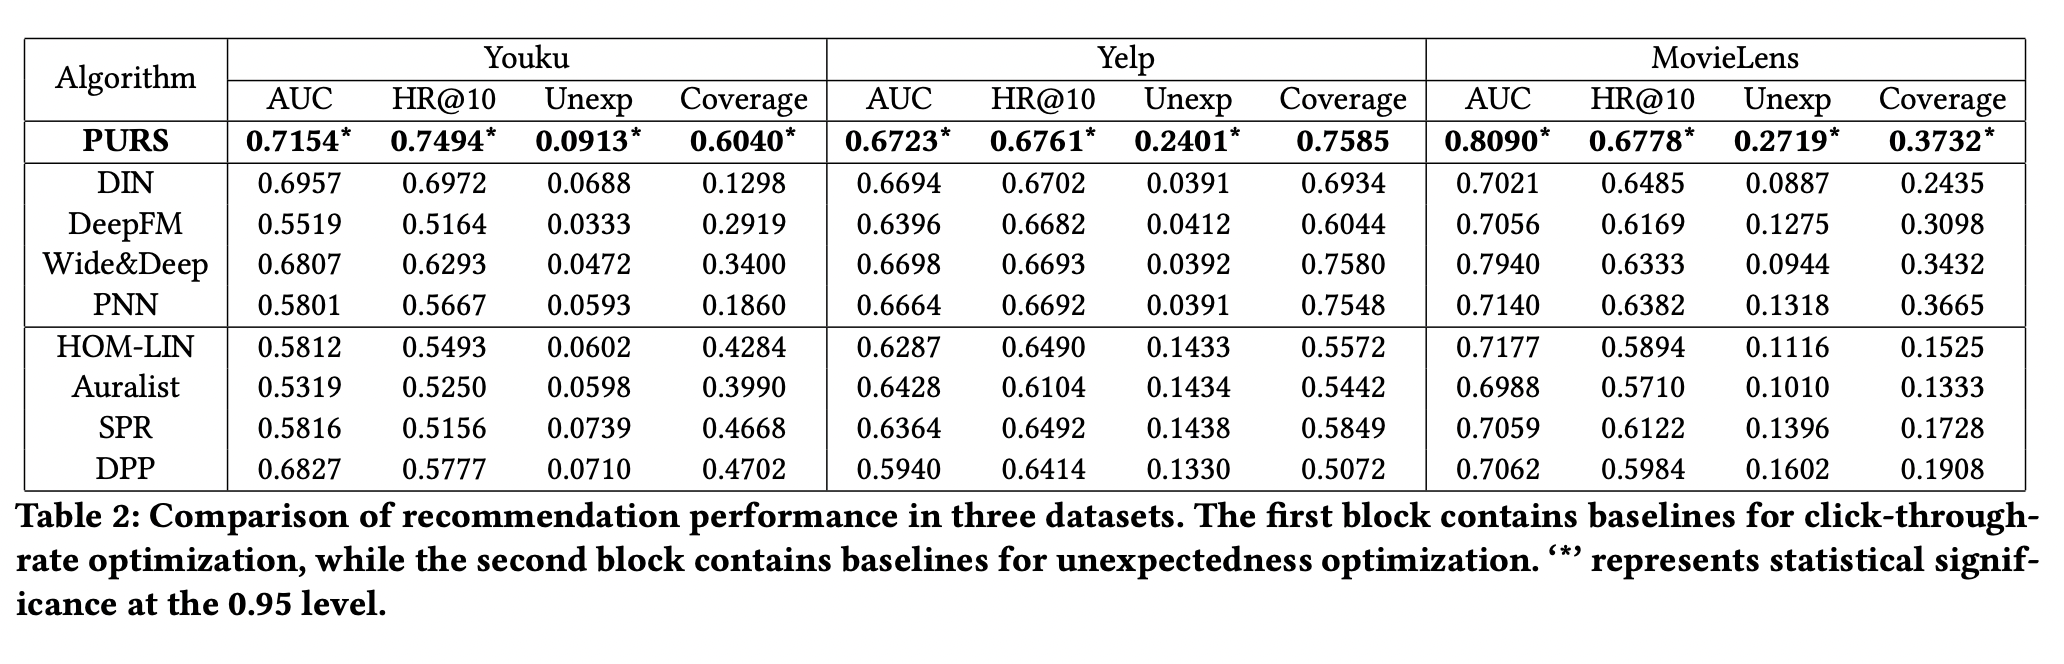
\includegraphics[width=100mm]{results.png}
    \caption{Results Comparison(from [1])
    \label{overflow}}
\end{table}
The PURS research team attributes the improvements to the following four factors: First, unexpectedness; Second, Unexpected Activation Function, which adjusts the input of unexpectedness into the utility function; Third, Personalized and Session-Based Factor, which encapsulates the user and session-level heterogeneity of perception towards unexpectedness; and finally Clustering of Behavior Sequence, which extracts the diverse user interests and constructs user expectations. Removal of any of these four components would result in a significant loss in both accuracy and unexpectedness measures. PURS is currently being deployed by Alibaba, a Chinese multinational technology company specializing in e-commerce, retail, Internet, and technology.
To conclude, the PURS model incorporates unexpectedness into the recommendation process. More precisely, user interests are represented as clusters of embedding closures in the latent space and unexpectedness is computed as the weighted distance between the new items and the interest clusters. Furthermore, the sequence modeling and the self-attention mechanism is implemented to represent personalized and session-based user perception of unexpectedness. Moreover, a novel unexpected activation function  is used in order to obtain improved unexpected recommendation performance. Finally, the CTR estimation is combined with the degree of unexpectedness to predict recommendations. The proposed PURS model surpasses baselines models both in terms of accuracy as well as novelty, successfully reducing the filter bubble effect. 

\section{A Framework for Recommending Accurate and Diverse Items  Using Bayesian Graph Convolutional Neural Networks}

The paper "A Framework for Recommending Accurate and Diverse Items  Using Bayesian Graph Convolutional Neural Networks" \footnote {Diversity in this paper means novelty} [2] introduces an alternative approach to deal with the filter bubble problem. Most existing recommender systems overlook diversity of the recommended list which leads to substandard performance. The model put forward in this paper is based on a Bayesian Graph Neural Network (BGNN). BGNNs enable the system to capture the uncertainty in the observed user-item interaction records while simultaneously bringing diversity into the recommendations.  Recently, BGNN based approaches have been used to capture the various relationships between a user and items while modeling user preferences in several personalized recommender system models. Most graph-based recommendation approaches depict the observed user-item interaction graph as a relationship between users and items resulting in sparse data. In these models, more often than not, all the unobserved user-item interactions are classified as negative samples. There are missing links that represent a given user’s possible future behavior. Also, there may be ambiguous positive interactions. To address the data sparsity issue, the researchers use Bayesian Graph Convolutional Neural Networks (BGCF) as a way to model the uncertainty in the user-item interaction graph. The BGNN incorporates a random graph generative model based on node-copying, which enables producing sample graphs similar to the observed graph. However, these graphs contain enough diversity to promote improved learning. To recap, the proposed model, BGCF, aims to tackle three big issues: 1) the sparsity issue, i.e. when user-item historical data is sparse, 2) the uncertainty issue, i.e when the data is noisy, and 3) the diversity issue, i.e. leading users to explore novel items. Currently graphs are used to model the relational data present in recommendation data sets. The user-item interaction can be represented as a bipartite graph.  The key idea in GCNs is to teach the model how to iteratively collect feature data from local graph neighborhoods using NNs.  Bayesian Personalized Ranking loss for Implicit Recommendation: The objective of the recommender system is to generate a  $total ranking>_u$ of all items for each user $u$. The graph attention network (GAT) uses self-attention operating on groups of spatially near neighbors to implicitly specify different weights for each node in a given neighborhood. The thinking behind this is that higher importance is placed on those neighbors that are more similar to the central node. GAT implemented a single-layer feedforward NN with multiple weights on sets of node feature vectors and on the transformation function to map from $\mathbb{R}^{2d}\longrightarrow\mathbb{R} $ as the attention score. Diversity (i.e. novelty) and accuracy metrics have conflicting interests: increasing one can negatively impact the other. The trade-off between diversity- in-top-$N$ and precision-in-top-$N$ is a major goal for this research. Concretely this means having a recommender system with a better accuracy/diversity trade-off leads to having more personalized recommendations without substantially sacrificing accuracy.

They show how their framework can be leveraged to infer providing a concrete formulation using the Bayesian Probabilistic Ranking training loss. As is evident in table 3.2, the testing on benchmark data sets has shown their model to be effective and to outperform state-of-the-art graph-based recommendation models. 

\begin{table}[hh!]
    \centering
    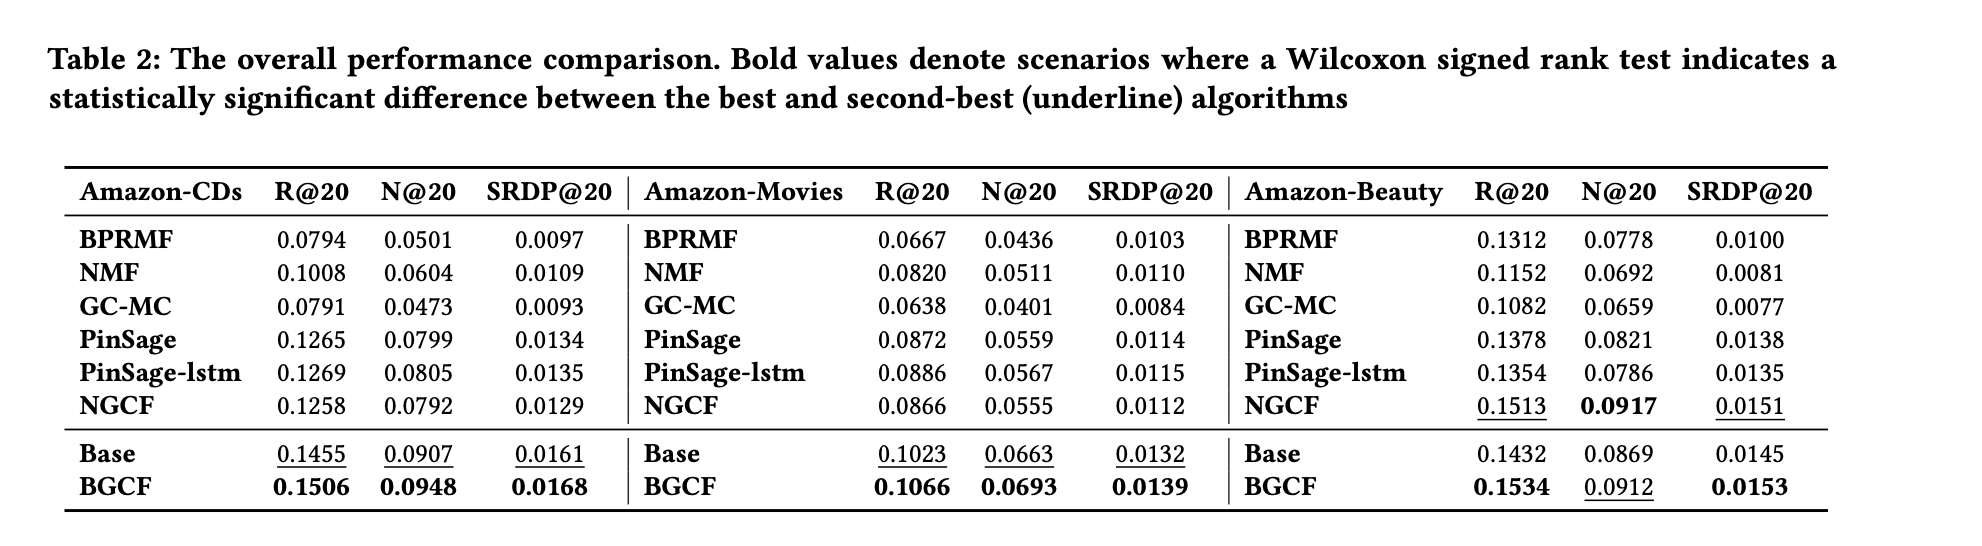
\includegraphics[width=125mm]{BGCF_results_comparison.png}
    \caption{Results Comparison (from [2])
    \label{overflow}}
\end{table}

The experiments were run on three benchmark datasets: Amazon-CDs, Amazon-Movies, and Amazon-Beauty. (Amazon-review\footnote{ http://jmcauley.ucsd.edu/data/amazon/} is a popular dataset for product recommendations: Three subsets are used here: Amazon-Movies, Beauty and CDs.) For all experiments, the recommendation accuracy of our model and baselines were assessed in terms of Recall@k and NDCG@k. Since accuracy alone does not guarantee user satisfaction, they also use serendipity@k, which factors in how surprising and relevant a recommendation is for a user. Moreover, they implement an all-scenario deep learning framework developed by Huawei, which can effectively be executed on multiple GPUs in parallel, drastically speeding up training.  Moreover, the proposed Bayesian Graph Collaborative Filtering framework incorporates diversity to the recommendations as well as alleviates the data sparsity challenges. The proposed model has the potential to be powerful for cold-start users in particular, offering a significant benefit in real-world recommender systems. 

\chapter{Multi-Armed Bandits}
According to Personalization Glossary [7] contextual bandits are defined as follows: "With the help of a relevant user data stream, contextual bandits for website optimization rely on an incoming stream of user context data, either historical or fresh, which can be used to make better algorithmic decisions in real time."
The multi-armed bandits solve the Exploration-Exploitation dilemma by striking a balance between exploration and exploitation of bandits, i.e. exploring arms which might be good and exploiting arms which are known to be good.

\section {Learning from Cross-Modal Behavior Dynamics with
Graph-Regularized Neural Contextual Bandit}

Contextual bandits is a variation of the multi-arm bandit problem. In addition to having a choice over arms, there is also a context vector. The features in the context vector include user data such as their age, the internet user behavior, etc. For each context, a choice has to be made over which arm to select. The process iterates until the best arm for each context is found[8]. In essence, the contextual multi-armed bandit problems are sequential decision problems with the goal to select the arm with the highest estimated reward in each trail, with the key idea being to learn a reward mapping function in order to infer the arm with the highest reward to pick. Many Contextual multi-armed bandit algorithms fall short of capturing complex, nonlinear inter-dependencies of user-item interactions. Additionally, these models often ignore the latent relations among users and non-recommended items, failing to properly reflect users’ preferences. Moreover, most existing approaches rely on historical data facing cold-start problems for new users with no previous user history. Learning from Cross-Modal Behavior Dynamics with Graph-Regularized Neural Contextual Bandit [4] describes an approach which focuses on resolving the aforementioned issues. The proposed Graph Regularized Cross-modal (GRC) learning model is extremely efficient in addressing and overcoming the cold-start problem. GRC is a general framework which exploits transferable data learned from user-item interactions and the external user-item features in online personalized recommendations. In particular, they exploit both positive and negative user-item interactions as well as unrecommended items through metric learning. GRC models complex user-item relationships using inherently nonlinear neural networks. Furthermore, the researchers augment GRC by combining the metric learning technique and a graph-constrained embedding module with the purpose of mapping different dimensions(temporal, social, and semantic) into the same latent space. GRC uses a multi-layer perceptron (MLP) module to grant the bandit algorithm of modelling non-linear structure of user-item relations. The great challenge is to directly derive the corresponding upper confidence bound for uncertainty estimation due to the dynamic nature in which context information is provided and the information not being strongly correlated with previous states and actions. To deal with this challenge, dropout layers are applied to learn the reward mapping function by unifying the strengths of neural network models and stochastic modeling. Also, to model the latent relations between users and items, they implement triangle inequality relation structures to capture the dependencies among positive, negative, and other unselected candidate user-item interactions. 
\begin{table}[hh!]
    \centering
    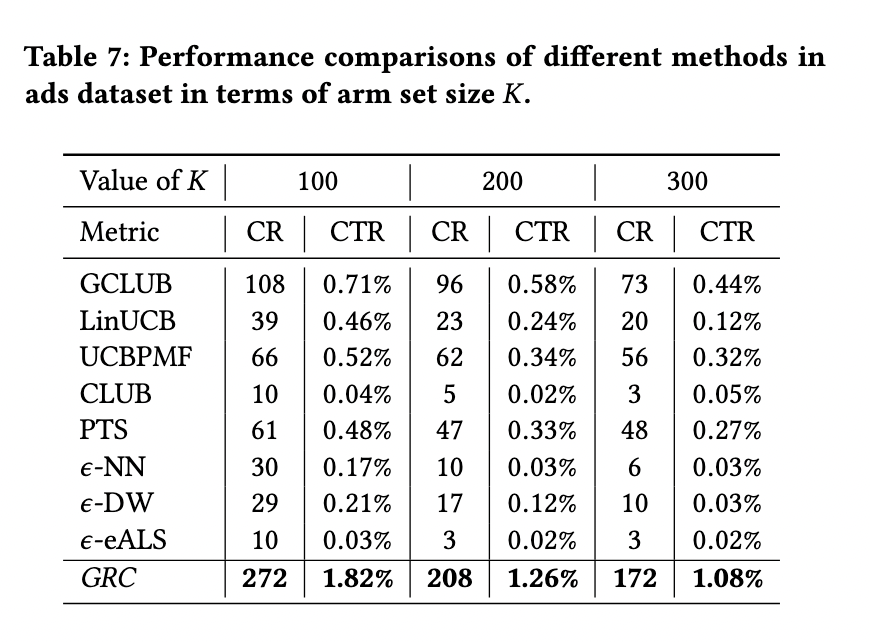
\includegraphics[width=100mm]{results_GRC.png}
    \caption{Results Comparison (from [4])
    \label{overflow}}
\end{table}
The model performance was assessed on three different datasets: 1) The LastFM Data, a dataset containing  users and artists (items) collected from a music streaming service website, 2) the Delicious Data, a social bookmarking web service data, and 3) Ads Click Stream Data, a proprietary ads click stream data from Yahoo Gemini platform. As table 4.1 shows, GRC performs better than the baselines \footnote {GCLUB, LinUCB, UCBPMF, CLUB, PTS, \textepsilon-NN, \textepsilon-DW,and \textepsilon-eALS} on all compared methods over different size of arm set. The results display the efficacy of the GRC model in capturing users’ dynamic preferences under changing settings and outperforming all baselines. The model is well-suited for capturing novel, latent, and complex user-item information.

\section{Deep Bayesian Bandits: Exploring in Online Personalized
Recommendations}
"Deep Bayesian Bandits: Exploring in  Online Personalized Recommendations" [3] offers a powerful solution to the feedback loop issue, addressing the problem of a recommender system acting greedily and favoring items already engaged by users. To combat algorithmic bias, causal inference and bandit theory and reinforcement learning (RL) are used. The model effectively employs bandit algorithms and posterior approximation algorithms for deep neural networks. Furthermore, they present a hybrid model that contains dropout units in the second-to-last layer. Confidence intervals are estimated in the UCB exploration. The proposed approach involves a trade-off between exploration and exploitation. Moreover, the exploration algorithm chooses K new items to introduce to a given user. Later, the neural network is fine-tuned using logged user actions for the predicted items. 

In addition to mitigating the filter bubble problem, Deep Bayesian Bandits is also effective against the cold-start problem. It does this by providing new information about the environment, including user preferences with the potential to result in  higher long-term rewards. More specifically, the researchers formulate a recommender as a contextual bandit problem and implement exploration techniques that require sampling from the posterior distribution -- summaries of what is known about uncertain quantities in Bayesian analysis-- of click-through-rates [4]. In their work, the researchers approximate uncertainty estimates of the predictions by implementing a bootstrapped model with multiple heads and dropout units. The context of the proposed model consists of user and item (ad) features. The model utilizes two distinct exploration algorithms: upper confidence bound(UCB) and Thompson sampling. To overcome the lack of an uncertainty estimate, they exploit neural networks, using dropout, bootstrapping, finally proposing a hybrid method that incorporates both dropout and bootstrapping. 

The model is tested following a continuous training and self-training setup. The offline model is based on Twitter data and ADS-16 dataset [26] is a publicly available dataset
that contains ratings of 300 ads shown to 120 users. The online experiments were run on a continuous data stream of 2\text{\%} of real time production traffic for 14 days. The online model was assessed on test data gathered by a random policy serving 1\text{\%} production traffic, which is representative of the distribution of the user-advertisement pairs.  Advertisement impressions are brought to users, and next, the label is published to a data stream the model’s training service is subscribing to. The model is warm-started from the previous version, and fine-tuned with newly collected data. For both the offline simulation and online simulations, the model is updated at regular intervals. The model is trained on self-generated data, forming a self-training loop. Both offline and online models were trained in a self-training loop using only data generated by that model. 

\begin{table}[hh!]
    \centering
    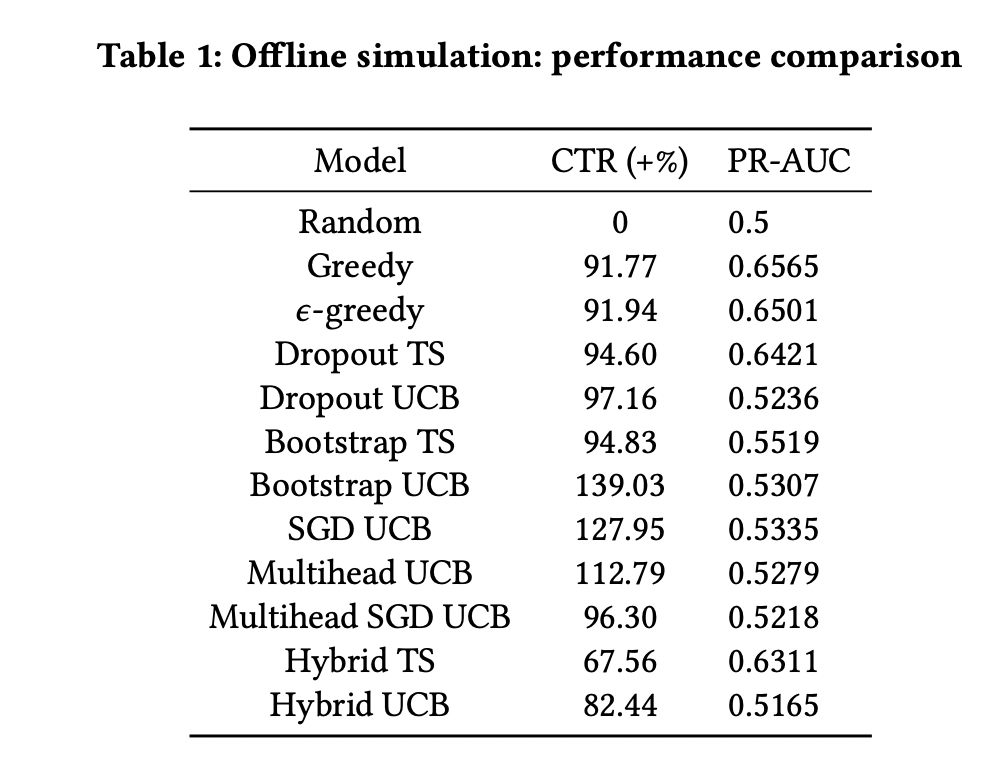
\includegraphics[width=100mm]{bandits_results.png}
    \caption{Results Comparison (from [3])
    \label{overflow}}
\end{table}

Table 4.2 shows the performance comparison in an offline experiment. For the offline simulation, a fully-connected feed-forward network. The Hybrid UCB earns more overall reward than the Hybrid TS. For example, CTR is 14.88 \text{\%}  higher for UCB than for Ts. Bootstrap UCB earns the highest rewards, but at the expense of having the highest computational cost. The performance drops with the reduction of
the computational cost of the Bootstrap UCB model by using other
variants, including the Hybrid model.
The results for the performed offline comparison
and online AB testing with large scale in-house data demonstrated high performance of the proposed model with a lower computational
cost. The model is able to address the algorithmic bias problem while simultaneously optimizing for users' long-term reward. 

\chapter{Personalized Transformer}
\section{SSE-PT Sequential Recommendation Via Personalized Transformer}

The Personalized Transformer (SSE-PT) [5] utilizes temporal data to find personalized recommendations, which is crucial for recommendation problems since user preferences in real life are dynamic in nature. Traditionally, recommender systems have primarily been based on standard collaborative filtering and ranking approaches rather than tracking sequential data. Recently, on top of powerful RNN and CNN models, attention mechanisms used in Natural Language Processing (NLP) enable the exploitation of the temporal ordering of items that users have engaged with. 
Especially the SASRec model based on the powerful NLP Transformer model has achieved impressive state-of-the-art results. Unfortunately, SASRec, is an unpersonalized model, lacking personalized user embeddings. SSE-PT is a personalized extension of the transformer model. It is sequence based, meaning that the model treats every sequence  as a given user's engagement history. The model achieves commendable results in capturing sequential, dynamic, and personalized user information. The proposed model addresses the limitations of the SASRec model outperforming it by almost 5$\%$ in terms of NDCG@10 on 5 real-world datasets. Moreover, a slightly modified SSE-PT model, which the researchers call SSE-PT++, can handle extremely long sequences, outperforming SASRec in ranking results with comparable training speed, striking a balance between performance and speed requirements. Moreover, their novel application of the Stochastic Shared Embeddings (SSE) regularization is essential to the success of personalization. Making use of user embeddings, the Personalized Transformer is able to capture a given user's recent engagement patterns. Personalization significantly improves ranking performance.
Sequential Recommendation means, "Given $n$ users with each user engaging with $m$ items in temporal order with the objective to learn a good personalized ranking of $K$ items." Sequences $s_i$ of length $T$ include indices of the most recent $T$ items that a user $i$ has interacted with in the temporal order

The application of Stochastic Shared Embeddings: Stochastic Shared Embeddings (SSE) are the most crucial regularization technique to the SSE-PT model, preventing the model from over-fitting badly after the introducing user embeddings. SSE refers to the process of 
stochastically replacing embeddings with another embedding with
a predefined probability during SGD\footnote{stochastic gradient descent}, which regularizes the embedding layers. 
\begin{table}[ht!]
    \centering
    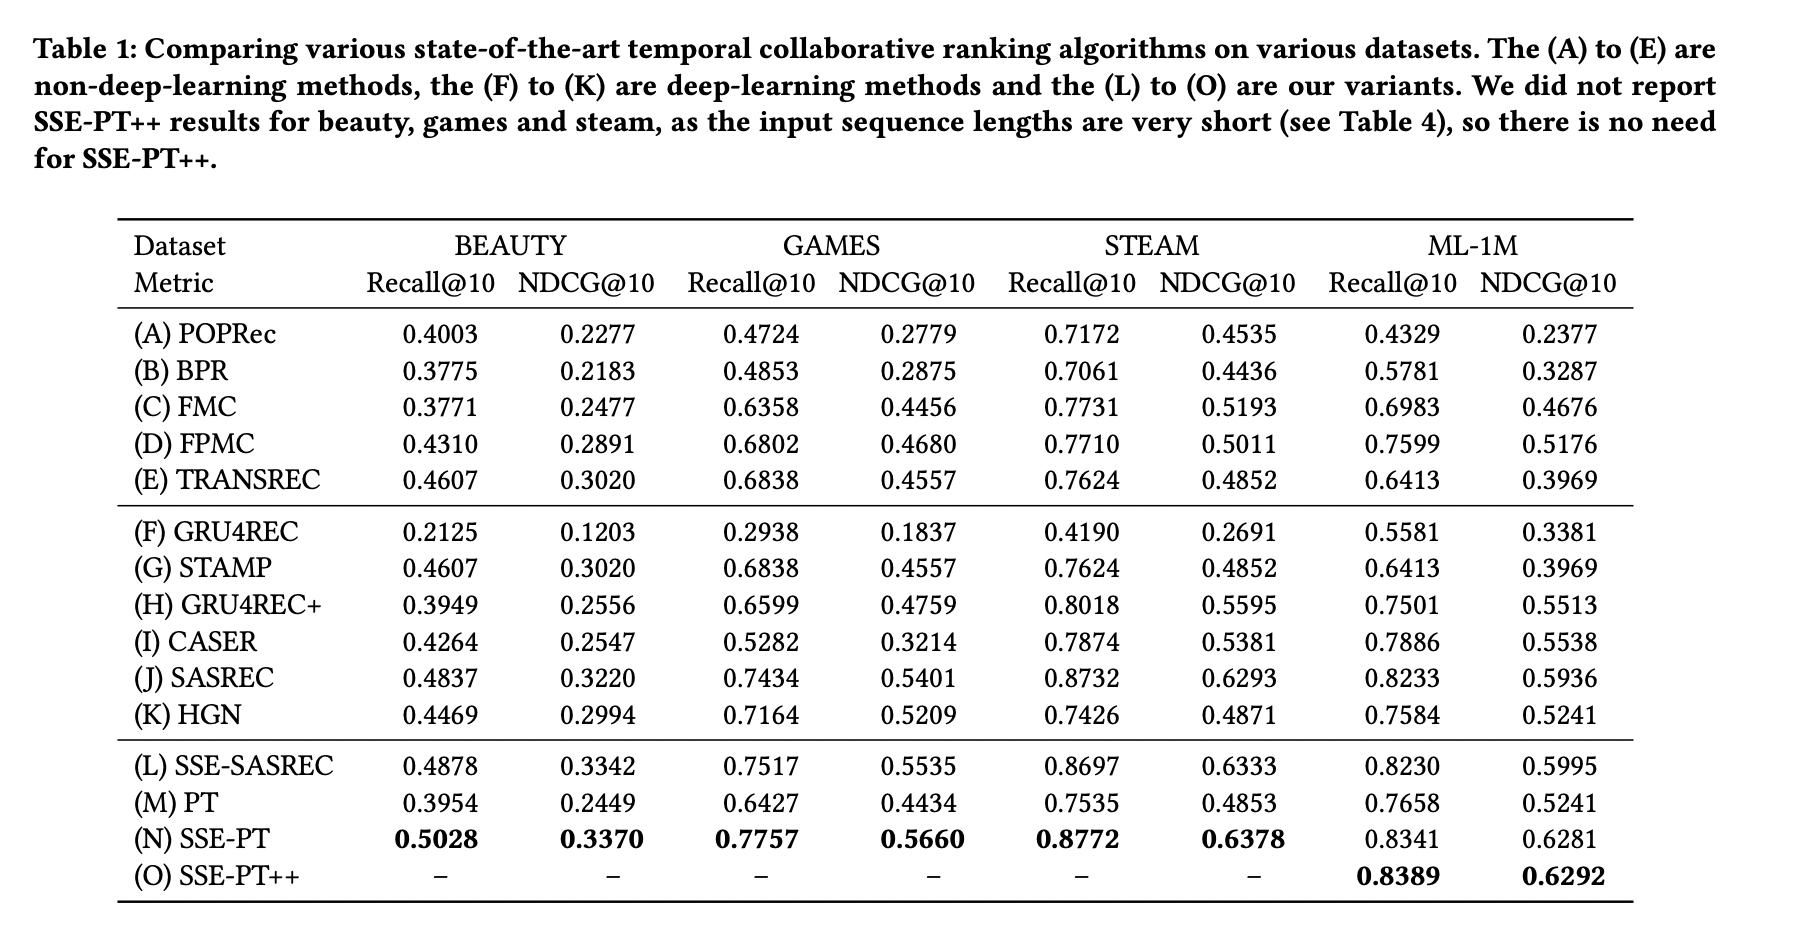
\includegraphics[width=100mm]{results_Transformer.png}
    \caption{Results Comparison (from[5])
    \label{overflow}}
\end{table}
The experiments were run on five datasets: 1) Amazon-Beauty, 2) Amazon-Games, 3) Steam -- a dataset containing reviews crawled from a large video game distribution platform, 4) Movielens 1M dataset -- a dataset containing one million user movie ratings, and 5) Movielens 10M dataset -- a dataset containing ten million user ratings cleaned by the researchers of this paper. For evaluation metrics, Normalized Discounted Cumulative Gain (NDCG) \footnote{NDCG is a popular method for measuring the quality of a set of search results} and Recall for top recommendations were used. We can see from Table 5.1 that the SSE-PT outperforms over all previous methods on the four datasets. Both SSE-PT and SSE-PT++ obtain notably better ranking performances than the baseline SASRec. SSE-PT helps mitigate the temporal collaborative ranking problem. On account of the attention mechanisms
during inference, the Personalized Transformer is also more interpretable and pays more attention to recent items in long sequences than the unpersonalized deep learning counterparts.

\chapter{ Conclusion}

All of the five models presented in this thesis have achieved remarkable results refining existing models. Effective recommender systems are vital to both businesses and individuals alike. Recommender systems help individuals in decision-making, guiding them to find interesting items in a huge pool of options. Using Recommender systems can help companies to increase their revenue and profit. The purpose of this thesis is to look into ways in which some recent, outstanding, cutting-edge recommender systems find solutions to common problems faced by current personalized recommender systems.

Modeling user interests as clusters of embedding closures while incorporating unexpectedness as the weighted distance between the novel items and the interest clusters, sequence modeling together with self-attention [1, 2, 5] as well as an adaptation of Transformer model with personalized embeddings have been shown to improve the quality of recommendations in personalized Recommender Systems. Two of the models discussed in sections  4.1. and 4.2 utilize multi-armed bandits to optimize recommendations. Furthermore, contextual bandits with deep neural networks, Bayesian Graph Neural Networks, and the use of graph-regularized cross-modal learning frameworks have proven to enhance the power of recommender systems. The five models enable efficient operations online, where new users or items arrive continually at an incredibly high rate, yielding significantly better recommendations for individual users than most existing recommender systems, providing original and potent solutions to major issues afflicting present recommender systems.